\documentclass[12pt,a4paper]{article}
\usepackage{geometry}
\geometry{left=2.5cm,right=2.5cm,top=2.0cm,bottom=2.5cm}
\usepackage[english]{babel}
\usepackage{amsmath,amsthm}
\usepackage{amsfonts}
\usepackage[longend,ruled,linesnumbered]{algorithm2e}
\usepackage{fancyhdr}
\usepackage{ctex}
\usepackage{array}
\usepackage{listings}
\usepackage{color}
\usepackage{graphicx}
\usepackage{amssymb}
\newtheorem{theorem}{定理}
\newtheorem{lemma}[theorem]{引理}
\newtheorem{corollary}[theorem]{推论}

\begin{document}
	
	\noindent
	
	\section*{2024.05.13}	
	
	\begin{enumerate}
		\item 如果 $K$ 是矩形, $P_K=Q_1(K)$, 证明如图所示的边的中点值所确定的节点参数对 $P_K$ 不是唯一可解的 (Hint 试着构造 $v \in Q_1(K)$ 使得 $\left.v\left(m_i\right)=0,1 \leq i \leq 4\right)$
		\begin{figure}[h]
			\centering
			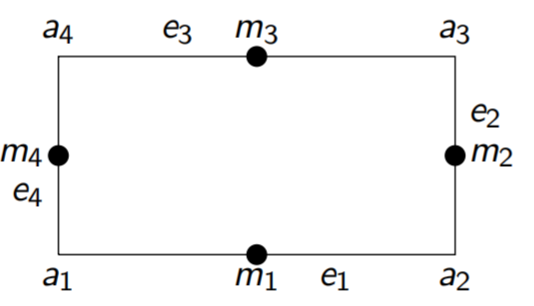
\includegraphics[width=0.7\linewidth]{rec}
			\label{fig:rec}
		\end{figure}
		
		\begin{proof}
			令$\xi=\frac{x-x_0}{\ell_1},\quad\eta=\frac{y-y_0}{\ell_2}.$
			
			考虑$v = \xi \eta$. 显然$v \in Q_1(K)$且$v(m_i)=0$,且$v \not\equiv 0$
		\end{proof}
		
		\item 如果 $K$ 是矩形, $P_K=\left\{1, x, y, \xi^2-\eta^2\right\}$, 证明 $\mathcal{N}_K=\left\{N_i, 1 \leq i \leq 4\right\}$,其中 $N_i(v)=\frac{1}{\left|e_i\right|} \int_{e_i} v \mathrm{ds}, 1 \leq i \leq 4$ 对 $P_K$ 是唯一可解的.
		
		\begin{proof}
			易得$P_K=\{1,\xi,\eta,\xi^2-\eta^2\}$,设$v = a_1 (\xi^2 - \eta^2) + a_2 \xi +a_3 \eta +a_4$.
			
			由$N_i(v) = 0, \quad i = 1,2,3,4$,可得
			$$\int_{-1}^1 -a_1 (1-\eta^2) + a_2 + a3\eta + a_4 d\eta =0$$
			$$\int_{-1}^1 -a_1 (1-\xi^2) + a_2 + a3\xi + a_4 d\xi =0$$
			$$\int_{-1}^1 -a_1 (1-\eta^2) - a_2 + a3\eta + a_4 d\eta =0$$
			$$\int_{-1}^1 -a_1 (1-\xi^2) - a_2 + a3\xi + a_4 d\xi =0$$
			
			即
			$$-\frac{2}{3}a_1+2(a_1+a_2+a_4)=0$$
			$$-\frac{2}{3}a_1+2(a_1+a_2+a_3)=0$$
			$$-\frac{2}{3}a_1+2(a_1-a_2+a_4)=0$$
			$$-\frac{2}{3}a_1+2(a_1-a_2+a_3)=0$$
			
			解得
			$$a_1=a_2=a_3=a_4 = 0$$
			
			从而$v \equiv 0$.
		\end{proof}
		\item 证明Morley有限元空间 $V_h$ 满足 $V_h \nsubseteq H^2(\Omega)$ 且 $V_h \nsubseteq H^1(\Omega)$
		
		Morley元的有限元空间:
		
		$V_h=\{v\in L^2(\Omega)\mid v|_K\in P_2(K),\forall K\in T_h,v$在$T_h$的所有顶点连续,
		$\frac{\partial v}{\partial\nu_\mathrm{e}}$在$\mathcal{T} _h$所 有 内 边 e的 中 点 连 续 $\}$
		
		\begin{proof}
			不妨设某条内边$e = (-1,0)\rightarrow(1,0)$,相邻单元为$K_1,K_2$.
			
			考虑$v |_ {K_1} = x^2-1,v |_ {K_2} = 1-x^2$.满足$v \in V_h$但$v \notin H^1(\Omega)$
		\end{proof}
		\item 验证课件中给出的函数是Morley元的节点基函数
		
		\begin{equation*}
			\begin{aligned}
				p_{i}=& 1-(\lambda_{i-1}+\lambda_{i+1})+2\lambda_{i-1}\lambda_{i+1}  \\
				&-\left(\nabla\lambda_{i-1}\right)^T\nabla\lambda_{i+1}\sum_{k=i-1,i+1}\frac{\lambda_k(\lambda_k-1)}{\left\|\nabla\lambda_k\right\|^2},\quad1\leq i\leq3 \\
				p_{i+3}=& \frac{\lambda_{i}(\lambda_{i}-1)}{\|\nabla\lambda_{i}\|},1\leq i\leq3. 
			\end{aligned}
		\end{equation*}
		
		\begin{equation*}
			\begin{aligned}
				N_i(v)=v(a_i),1\leq i\leq3\\N_{i+3}(v)=\frac{\partial v}{\partial\nu}(m_i),1\leq i\leq3
			\end{aligned}
		\end{equation*}
		
		$$a_1 = (1,0,0),a_2=(0,1,0),a_3=(0,0,1)$$
		$$m_1 = (0,0.5,0.5),m_2=(0.5,0,0.5),m_3=(0.5,0.5,0)$$
		
		\begin{proof}
			
			
			注意到$\nabla \lambda_i = \frac{1}{2|S_K|} (y_j-y_k,x_k-x_j)$,$e_i=(x_k-x_j,y_k-y_j)$.从而$-\nabla \lambda_i ^\top$为$e_i$ 的外法向量,$-\frac{\nabla \lambda_i}{\|\nabla \lambda_i\|}^\top$为$e_i$的单位外法向量$\nu_{e_i}$。
			
			$$N_1(p_1) = 1-(0+0)+2*0*0-0 = 0$$
			$$N_1(p_2) = 1- (1+0) - 2*1*0 - 0 = 0$$
			$$N_1(p_4) = \frac{0}{\|\nabla \lambda_1\|} = 0$$
			
			计算得
			$$
			\nabla p_{k}=\Big(-\nabla\lambda_i-\nabla\lambda_j+2(\lambda_i\nabla\lambda_j+\lambda_j\nabla\lambda_i)-\nabla\lambda_i^\top\nabla\lambda_j\sum_{k=i,j}\frac{(2\lambda_k-1)\nabla\lambda_k}{\|\nabla\lambda_k\|^2}\Big) \quad k = 1,2,3
			$$
			\begin{equation*}
				\begin{aligned}
					N_4(p_1) = \nabla p_1 (m_1) \cdot \nu_{e_1} = 0 \cdot \nu_{e_1} = 0
				\end{aligned}
			\end{equation*}
			\begin{equation*}
				\begin{aligned}
					N_4(p_2) &= \nabla p_2 (m_1) \cdot \nu_{e_1} \\
					&=\Big( -\nabla\lambda_{2}+\nabla\lambda_{1}^{\top}\nabla\lambda_{2}\frac{\nabla\lambda_{1}}{\|\nabla\lambda_{1}\|^{2} } \Big) \cdot  \Big(-\frac{\nabla \lambda_1}{\|\nabla \lambda_1\|}\Big)^\top\\
					&= 0.  (\text{利用单位外法向量})
				\end{aligned}
			\end{equation*}
			
			计算得
			$$\nabla p_{i+3}=\frac{1}{\|\nabla\lambda_i\|}(2\lambda_i-1)\nabla\lambda_i \quad i = 1,2,3$$
			\begin{equation*}
				\begin{aligned}
					N_4(p_4) = \nabla p_4(m_1) \cdot \nu_{e_1} = \Big(-\frac{\nabla \lambda_i}{\|\nabla \lambda_i\|}\Big)^\top\cdot \Big(-\frac{\nabla \lambda_i}{\|\nabla \lambda_i\|}\Big) = 1
				\end{aligned}
			\end{equation*}
			$$N_4(p_5) = \nabla p_5 (m_1) \cdot \nu_{e_1} = 0 \cdot \nu_{e_1} = 0$$
			
			结合对称性,验证完毕。
		\end{proof}
	\end{enumerate}
	
	
\end{document}

